%% This is file `sample-acmsmall.tex',
%% generated with the docstrip utility.
%%
%% The original source files were:
%%
%% samples.dtx  (with options: `acmsmall')
%% 
%% IMPORTANT NOTICE:
%% 
%% For the copyright see the source file.
%% 
%% Any modified versions of this file must be renamed
%% with new filenames distinct from sample-acmsmall.tex.
%% 
%% For distribution of the original source see the terms
%% for copying and modification in the file samples.dtx.
%% 
%% This generated file may be distributed as long as the
%% original source files, as listed above, are part of the
%% same distribution. (The sources need not necessarily be
%% in the same archive or directory.)
%%
%%
%% Commands for TeXCount
%TC:macro \cite [option:text,text]
%TC:macro \citep [option:text,text]
%TC:macro \citet [option:text,text]
%TC:envir table 0 1
%TC:envir table* 0 1
%TC:envir tabular [ignore] word
%TC:envir displaymath 0 word
%TC:envir math 0 word
%TC:envir comment 0 0
%%
%%
%% The first command in your LaTeX source must be the \documentclass
%% command.
%%
%% For submission and review of your manuscript please change the
%% command to \documentclass[manuscript, screen, review]{acmart}.
%%
%% When submitting camera ready or to TAPS, please change the command
%% to \documentclass[sigconf]{acmart} or whichever template is required
%% for your publication.
%%
%%
% \documentclass[acmsmall]{acmart}
\documentclass[acmsmall,manuscript, screen, review]{acmart}
% \documentclass[acmsmall]{acmart}
% \usepackage{ragged2e} % don't use it
% \usepackage{bigstrut} % don't use
\usepackage{multirow}
\usepackage{float} 
\usepackage{subcaption}
 

%%
%% \BibTeX command to typeset BibTeX logo in the docs
\AtBeginDocument{%
  \providecommand\BibTeX{{%
    Bib\TeX}}}

%% Rights management information.  This information is sent to you
%% when you complete the rights form.  These commands have SAMPLE
%% values in them; it is your responsibility as an author to replace
%% the commands and values with those provided to you when you
%% complete the rights form.
\setcopyright{acmcopyright}
\copyrightyear{2018}
\acmYear{2018}
\acmDOI{XXXXXXX.XXXXXXX}


%%
%% These commands are for a JOURNAL article.
\acmJournal{JACM}
\acmVolume{37}
\acmNumber{4}
\acmArticle{111}
\acmMonth{8}

%%
%% Submission ID.
%% Use this when submitting an article to a sponsored event. You'll
%% receive a unique submission ID from the organizers
%% of the event, and this ID should be used as the parameter to this command.
%%\acmSubmissionID{123-A56-BU3}

%%
%% For managing citations, it is recommended to use bibliography
%% files in BibTeX format.
%%
%% You can then either use BibTeX with the ACM-Reference-Format style,
%% or BibLaTeX with the acmnumeric or acmauthoryear sytles, that include
%% support for advanced citation of software artefact from the
%% biblatex-software package, also separately available on CTAN.
%%
%% Look at the sample-*-biblatex.tex files for templates showcasing
%% the biblatex styles.
%%

%%
%% The majority of ACM publications use numbered citations and
%% references.  The command \citestyle{authoryear} switches to the
%% "author year" style.
%%
%% If you are preparing content for an event
%% sponsored by ACM SIGGRAPH, you must use the "author year" style of
%% citations and references.
%% Uncommenting
%% the next command will enable that style.
%%\citestyle{acmauthoryear}


%%
%% end of the preamble, start of the body of the document source.
\begin{document}

%%
%% The "title" command has an optional parameter,
%% allowing the author to define a "short title" to be used in page headers.
\title{ViST: A Ubiquitous Model with Multimodal Fusion for Crop Growth Prediction}

%%
%% The "author" command and its associated commands are used to define
%% the authors and their affiliations.
%% Of note is the shared affiliation of the first two authors, and the
%% "authornote" and "authornotemark" commands
%% used to denote shared contribution to the research.
\author{Junsheng Li}
% \authornote{Both authors contributed equally to this research.}
\email{22s103187@stu.hit.edu.cn}
\orcid{0000-0002-7724-7787}
% \authornotemark[1]

\affiliation{%
  \institution{Department of Computer Science and Technology, Harbin Institute of Technology}
  \streetaddress{No. 92, Xidazhi Street, Nangang District}
  \city{Harbin}
  \state{Heilongjiang Province}
  \country{China}
  \postcode{150000}
}

\author{Ling Wang}
\email{wangling@hit.edu.cn}
\affiliation{%
  \institution{Department of Computer Science and Technology,Harbin Institute of Technology}
  \streetaddress{No. 92, Xidazhi Street, Nangang District}
  \city{Harbin}
  \state{Heilongjiang Province}
  \country{China}
  \postcode{150000}
}


\author{Jie Liu}
\email{jieliu@hit.edu.cn}
\affiliation{%
  \institution{Department of Computer Science and Technology,Harbin Institute of Technology}
  \streetaddress{No. 92, Xidazhi Street, Nangang District}
  \city{Harbin}
  \state{Heilongjiang Province}
  \country{China}
  \postcode{150000}
}

\author{Jinshan Tang}
\email{jtang25@gmu.edu}
\affiliation{%
  \institution{Health Informatics, College of Public Health,George Mason University}
  \city{Fairfax}
  \state{VA}
  \country{USA}
  \postcode{22033}
}

%%
%% By default, the full list of authors will be used in the page
%% headers. Often, this list is too long, and will overlap
%% other information printed in the page headers. This command allows
%% the author to define a more concise list
%% of authors' names for this purpose.
\renewcommand{\shortauthors}{Junsheng et al.} % 页眉右上角

%%
%% The abstract is a short summary of the work to be presented in the
%% article.
\begin{abstract}
  Crop growth prediction can help agricultural workers to make accurate and reasonable decisions on farming activities. Existing crop growth prediction models focus on one crop and train a single model for each crop. In this paper, we will develop a ubiquitous growth prediction model for multiple crops, aiming to train a single model for multiple crops. A ubiquitous vision and sensor transformer(ViST) model for crop growth prediction with image and sensor data is developed to achieve the goals. In the proposed model, a cross-attention mechanism is proposed to implement the fusion of multimodal feature maps for reducing the computational cost and balancing the interactive effects between features. For training the model, we combine the data from multiple crops to train a single (ViST) model. A sensor network system is constructed for the data collection on the farm that plants rice, soybean, and maize. Experiment results show that the proposed ViST model has an excellent ubiquitous ability for crop growth prediction with multiple crops.
\end{abstract}

%%
%% The code below is generated by the tool at http://dl.acm.org/ccs.cfm.
%% Please copy and paste the code instead of the example below.
%%
\begin{CCSXML}
  <ccs2012>
  <concept>
  <concept_id>10010147.10010178</concept_id>
  <concept_desc>Computing methodologies~Artificial intelligence</concept_desc>
  <concept_significance>500</concept_significance>
  </concept>
  </ccs2012>
\end{CCSXML}

\ccsdesc[500]{Computing methodologies~Artificial intelligence}

%%
%% Keywords. The author(s) should pick words that accurately describe
%% the work being presented. Separate the keywords with commas.

\keywords{crop growth prediction,ubiquitous model, multimodal learning, transformer module,cross-attention mechanism}

\received{20 February 2007}
\received[revised]{12 March 2009}
\received[accepted]{5 June 2009}

%%
%% This command processes the author and affiliation and title
%% information and builds the first part of the formatted document.
\maketitle

\section{Introduction}
With the development of new technologies such as the Internet of things, big data, and artificial intelligence (AI), modern agriculture has been dramatically changed. One major task in modern agriculture is to predict crop growth. Crop growth prediction is used as the weather vane for agricultural activities. Accurate short-range prediction of crop growth can help farmers manage fertilization, irrigation, and pesticide spraying effectively. With the effective management of these agricultural activities, human and material resources can be reduced as much as possible, and the final yields and economic benefits can be significantly improved. It can also reduce the use of pesticides that pollute the environment and thus protect the ecological environment. 

There are many existing crop models for crop growth and yield prediction \cite{book,BRISSON2003309,boogaard1998wofost}. However, These models are designed for a specific crop and specific region and condition, which are not universal models. These models cannot be adaptive to any specific crop in different regions. The parameters and driving variables of the models are derived from the situation of a particular location, which can be measured and available under ideal conditions. Due to the inherent soil heterogeneity and the influence of farming methods on soil properties, the measured parameters will also be different. Because the biological system is too complex and many processes involved have to be fully understood, a universal model based on biology is different to build. A data-driven model with Neural Network makes it possible to build a universal model. Under the depth learning model, any dynamic systems, including crop systems, can be approximated through the design of network depth. 

In the past, a lot of research has focused on multi-scale crop images collected by UAV or satellite remote sensing for crop growth and yield prediction \cite{wang_new_2022,yue_estimate_2019,turkoglu_crop_2021}
. These image data reflect the phenotype characteristics of crops. The dynamic changes of crop phenotypes, such as the Leaf Area Index, are used to predict crop growth for a large region. Some researchers combine crop spectral data and soil and meteorological data for crop growth prediction \cite{trnka_effect_2007,islam_deep_2018,adisa_application_2019,liu_neural_2001,matsumura_maize_2015}
. However, these data-driven methods still need to be universal. The results are strongly related to collecting high-precision crop parameters and input data of crop environment. The processing of the data collection is costly, leading to the use for farm management hardly. 

To approximate the objective function, a model has to be built to apply to multimodal and multi-dimension data. Most existing multimodal mechanisms exist in automotive drive and medical fields \cite{guo2019deep,xiao2020multimodal}. Our work is the first to fuse crop RGB image and sensor data for low-cost crop growth prediction on farms. The multimodal fusion process fuses information from two or more modalities to realize information complementation and broaden the coverage of information contained in the input data. Different from other fields, the estimation model for crop growth by multimodal fusion has more challenges in generalization as each crop has its character. To solve this problem, we propose the ViST (Vision and Sensor Transformer) model, which can realize efficient information fusion for accurate prediction of crop growth.

Besides the fusion of multiple data resources for crop growth, we also investigate the possibility of hybrid training, which aims at developing a single network to predict the crop growth of multiple crops. In the past, many models for crop growth prediction were developed. However, all of these models were trained using a single crop, which means each crop needs a single model. On a farm, there are generally many crops. If each crop needs a trained model, training is time-consuming and complex for farmers to use. Thus, this paper aims to develop a ubiquitous model that could be used for multiple crops. A sensor network system is constructed for the data collection on the farm that plants rice, soybean, and maize.

The main contributions of this paper are as follows:

•	We proposed a ViST (Vision and Sensor Transformer) model for crop growth, which can efficiently utilize a multimodal data fusion mechanism. 

•	We also investigated the possibility of hybrid training, which aims at developing a single network to predict crop growth of multiple crops.  

•	The proposed model was compared with other existing models using real data from farms we collected, and the proposed model can obtain better performance than other existing models.



\section{Related Work}
\subsection{Single-modality approaches for crop growth prediction}
Single-modality approaches for crop growth prediction include two types of approaches: image-only and non-image sensor-only approaches. Image-based remote sensing technology for crop growth prediction is one of the image-only approaches. Image-based remote sensing technology has attracted attention as it can estimate crop growth effectively due to its ability to provide timely, dynamic, and macro-scale observations \cite{__2016}. With the development of machine learning techniques, image-based remote sensing technology for crop growth has developed further. They are often combined with machine learning techniques to estimate crop growth \cite{johnson_crop_2016,zhong_deep_2019,yang_deep_2019}. However, the quality of images acquired through traditional remote sensing is often affected by weather and cloud changes and thus affects the prediction. Besides, remote sensing technology generally has high maintenance and operation costs, affecting its vast uses. Recently, convenient image-based techniques, based on UAV drew the researchers’ attention\cite{weiss_plant_2011,tao_estimation_2020,zhou_predicting_2017,maimaitijiang_unmanned_2017,wan_grain_2020}. By mounting a camera to a UAV, high spatial resolution images of crops can be acquired and thus can be used for crop growth estimation. These techniques are beneficial for small farms. 

Non-image sensor-only approaches are also popular for growth prediction. Because crop growth is affected by climate/weather and soil conditions \cite{fortin_site-specific_2011,campbell_effect_1988,ehret_neural_2011}, thus meteorological and soil sensors have been widely used to predict crop growth attributes. These non-image sensor-only approaches often use machine learning techniques. Dahikar et al. \cite{dahikar_agricultural_2014} proposed a crop prediction method by sensing various soil parameters and parameters related to the atmosphere and using ANN for crop yield prediction in rural areas. O'Neal et al. \cite{oneal_neural_2002} designed a fully connected network to predict maize yield using local crop stage weather data and yield data from 1901 to 1996. Morimoto et al. \cite{morimoto_dynamic_2007} used a deep learning model to identify changes in citrus sugar and citric acid content based on rainfall and sunshine duration data. Drummond et al. \cite{drummond_application_1998} applied feedforward neural networks to estimate nonlinear relationships between soil parameters and crop yields. Kitchen et al. \cite{kitchen_soil_2003} found that neural networks could provide the most accurate empirical model of the data and fit the yield data well to soil and terrain features.


\subsection{Multimodal learning for crop growth prediction}
Image-only and non-image sensor-only approaches have shown impressive results in predicting crop growth \cite{padilla_proximal_2018}. However, regarding the integrity of information expression, the model obtained by a single modality still has certain defects for missing information. One solution is to integrate the representations of these two modalities to take advantage of their complementary advantages in crop growth prediction. 

Many deep learning-based approaches have been developed to handle multimodal data \cite{sengupta_review_2020}. Multimodal machine learning has led to a wide range of applications: from audiovisual speech recognition (AVSR)\cite{yuhas_integration_1989}, multimedia content indexing and retrieval \cite{snoek_multimodal_2005}, understanding human multimodal behavior, multimodal emotion recognition \cite{chen_heu_2021}, image and video captioning \cite{lei_video_2021}, VQA\cite{long_improving_2021}, multimedia retrieval \cite{souza_online_2021}, to health analytics \cite{yazdavar_multimodal_2020}, etc. Huang et al. \cite{huang_what_2021} proved from a theoretical point of view that multimodal learning could fuse the information of single modalities and complement each other so that the final effect of the model is better than that of a single modality.

In agriculture, there is some research on multimodal learning. Dang et al. \cite{dang2021autumn} used DNN with a multilayer feedforward perceptron(MLP) model for crop yield prediction. Chu et al. \cite{chu_end--end_2020} proposed an end-to-end prediction model for summer and winter rice yield based on MLP deep learning fusion. Two simple MLPS were used to extract spatial and temporal features, and then these two simple MLP models were combined to mine the relationship between features and rice yield. The model maintained stable convergence after 100 iterations. Maimaitijiang et al. \cite{maimaitijiang_soybean_2020} tried to use multimodal data fusion to complete tasks related to crop growth. The combined multimodal information, such as canopy spectral, structural, thermal, and texture features, are extracted. Input-level and middle-level feature fusion by MLP are used to predict crop grain yield. 

However, the previous work uses MLP for data fusion in the NN models. The problem is that it is suitable for small-scale learning. When the model scale is enlarged, it will suffer from serious overfitting. Due to the large amount of data in images, it is difficult for MLP to extract features efficiently \cite{zhao_battle_2021}. In addition, the learning efficiency of fully connected architectures is very low, which has long been confirmed by machine learning experiments. Inefficiency means that more training data are needed to reach a certain level of performance. Many application scenarios cannot provide enough data support, so it is necessary to introduce assumptions to improve the utilization efficiency of limited data. Therefore, the application scenarios of the fully connected architecture are limited, and there are also problems of poor interpretability and robustness.

With the success of Transformers and self-supervised learning, there has been increasing research on cross-modal learning, such as vision-language pre-trained models (VLP)\cite{clevers_remote_2013}, images and lidar fusion\cite{prakash_multi-modal_2021}, Audio set, Epic-Kitchens, and VGGSound classification \cite{nagrani_attention_nodate}. The attention adaptively generated by Transformer has good adaptability. Attention can filter out a small amount of important information from a large amount of data, focus on this vital information, and ignore the most unimportant information. The information is critical, and more weight can be assigned. That is, the weight represents the importance of the data \cite{vaswani_attention_2017}.

The multimodal fusion process fuses information from two or more modalities to realize information complementation and broaden the coverage of information contained in the input data. However, it inevitably adds much redundant information. Therefore, a more effective way of information fusion and expression is needed.

A multimodal learning method based on Transformer is proposed to complete the task of crop growth prediction. Compared with MLP, Transformer can extract features efficiently on tasks with a large amount of data, such as images and sensors. As a result, unnecessary calculations are reduced, and the efficiency and robustness of the prediction model are improved. A self-attention mechanism is proposed for fusing agricultural sensor and image data with fewer redundancy calculations. 

\section{Vision-and-Sensor Transformer model}

The proposed ViST overall network structure is shown in Figure \ref{model_structure}. The inputs are crop images and sensor data. In the framework, the MLP module and Linear Projection Flattened Patches module(LPFP) extract feature from sensor and image data, respectively. The transformer encoder is designed for data fusion. Pooler and Linear modules are intended to reduce the dimension of features.

\begin{figure}[htbp]
  \centering
  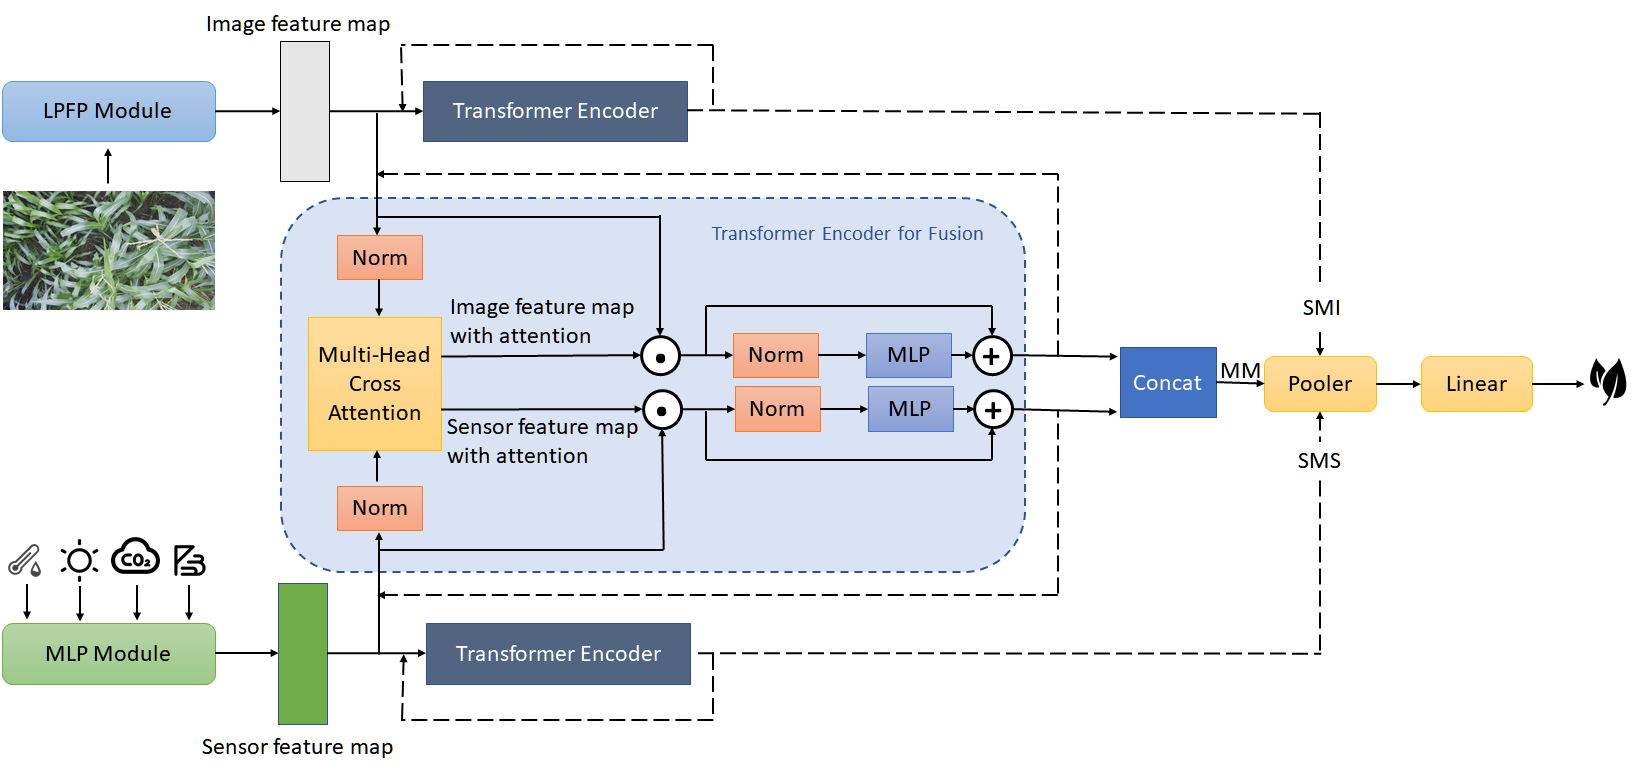
\includegraphics[width=\linewidth]{pic/model_structure.png}
  \caption{The framework of ViST for growth prediction.}
  \Description{This structure can obtain crop growth estimation through image-only, sensor-only, and multimodal input.}
  \label{model_structure}
\end{figure}
The input of the ViST is sensor and image data. They are processed independently at MLP and LPFP modules, respectively. The features from the two modules are input to one Transformer Encoder for feature fusion. The output of the encoder is given to the Concat module with the output for Multiple Modalities (MM). At the same time, the features are sent separately to the other two Transformer encoders for self-attention mechanics. The output of these two transformer encoders with cross-attention mechanics are Single Modality with Image(SMI) and Single Modal with Sensor(SMS), respectively. The output MM, SMI, and SMS are then input into the Pooler module to reduce the dimension of the features. Finally, the features were input to the linear layer module to output the leaf area index (LAI) value (in the range of [0,1]). The specific details of each module in the framework is described below.



\subsection{MLP Module}
Generally speaking, image data has three channels for RGB, and each pixel has a value. But sensor data only has dozens of values. Therefore, the number of values for Sensor data is much less than those for image data. Image data will dominate if the two data types are directly integrated; At the same time, the sensor data will not be well expressed.

To solve this problem, sensor data was converted into feature maps. MLP module can amplify the characteristics of the sensor data. The sensor data are composed of weather data and soil data. The data are numerical and have 19 data items. After data preprocessing, the sensor data were arranged into one-dimensional vectors and input into the multilayer feedforward perceptron(MLP) module. The MLP module is a multilayer perceptron that contains 19 neurons in the input layer and 768 neurons in the output layer. The specific structure of the MLP module is shown in Figure \ref{mlp_module}. The two hidden layers contain 32 and 64 neurons, respectively.
\begin{figure}[htbp]
  \centering
  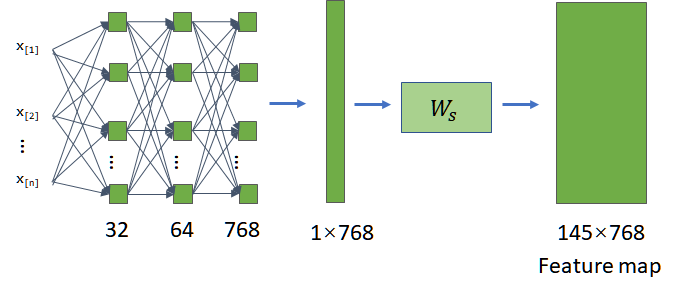
\includegraphics[width=0.7\linewidth]{pic/mlp_module.png}
  \caption{MLP Module.}
  \Description{Image and sensor input model structure.}
  \label{mlp_module}
\end{figure}

After the MLP module outputs a one-dimensional vector containing 768 elements, the size of the vector is 1\begin{math}
  \times
\end{math}768. This 1\begin{math}
  \times
\end{math}768 vector will be converted to a 145 x768 matrix using the following equation
\begin{equation}
  M_{out}=W_s\times M_{in}
\end{equation}
where \begin{math}
  M_{in}
\end{math} is the 1\begin{math}
  \times
\end{math}768 vector from ML module and the output \begin{math}
  M_{out}
\end{math} is a 145\begin{math}
  \times
\end{math}768 matrix.\begin{math}
  W_s
\end{math} is a matrix with a size of 145\begin{math}
  \times
\end{math}1. The element of \begin{math}
  W_s
\end{math} is obtained by training. 

In this paper, the sensor data is mapped to the same dimension as the image features of the LPFP module to facilitate subsequent feature fusion operations. It is worth noting that the sensor features based on the MLP module do not require position information, and the input order of sensor data can be arbitrarily scrambled.

\subsection{Linear Projection Flattened Patches module}
\begin{figure}[htbp]
  \centering
  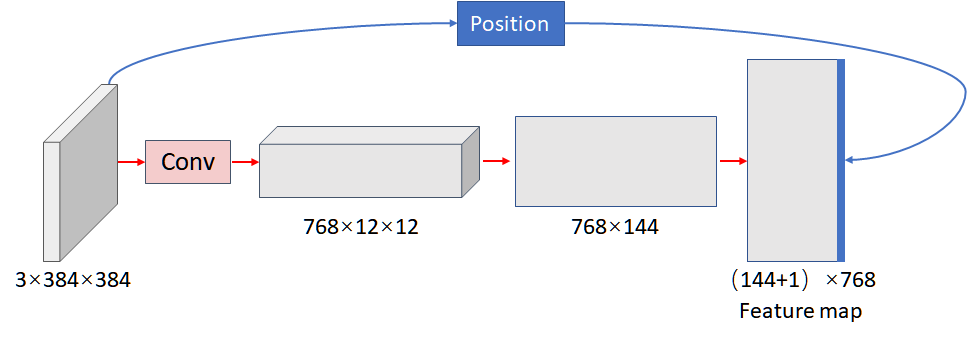
\includegraphics[width=0.7\linewidth]{pic/linear_projection_flattened_patches_module.png}
  \caption{Linear Projection Flattened Patches module.}
  \Description{Create image feature.}
  \label{linear_projection}
\end{figure}
The structure of the linear projection flattened patches module is shown in Figure \ref{linear_projection}. The input of the module is an image with a size of  CHANEL\begin{math}\times\end{math}HEIGHT\begin{math}\times\end{math}WIDTH (C\begin{math}\times\end{math}H\begin{math}\times\end{math}W). The 3D tensor corresponds to an RGB image. Before inputting the image, the image is adjusted to the size of 3\begin{math}\times\end{math}384\begin{math}\times\end{math}384, as shown in the input in Figure \ref{linear_projection}. The image is divided into 768 12\begin{math}\times\end{math}12 image blocks by 768 32\begin{math}\times\end{math}32 convolution cores and 32 convolution operation steps. Each small image is flattened into 144 one-dimensional vectors, and 768 flattened one-dimensional vectors are successively connected into 768\begin{math}\times\end{math}144 vectors. The 768\begin{math}\times\end{math}144 vectors is transposed to the 144\begin{math}\times\end{math}768 vectors to be fused with the feature vector from the sensor. Then, the 144\begin{math}\times\end{math}768 feature vector is spliced with the position information vector to generate 145\begin{math}\times\end{math}768 image features with position information. Linear Projection Flattened Patches divide the image into several equal small images and align the image feature map with the sensor features through matrix transformation. 

The image and sensor feature vectors are stacked together to form a sequence of the same dimensions, forming a compact representation of the environment encoded by the global context. The stacked vectors are ready to be input to the next transformer encoder for complete feature fusion. 


\subsection{Transformer Encoder for fusion}
\begin{figure}[htbp]
  \centering
  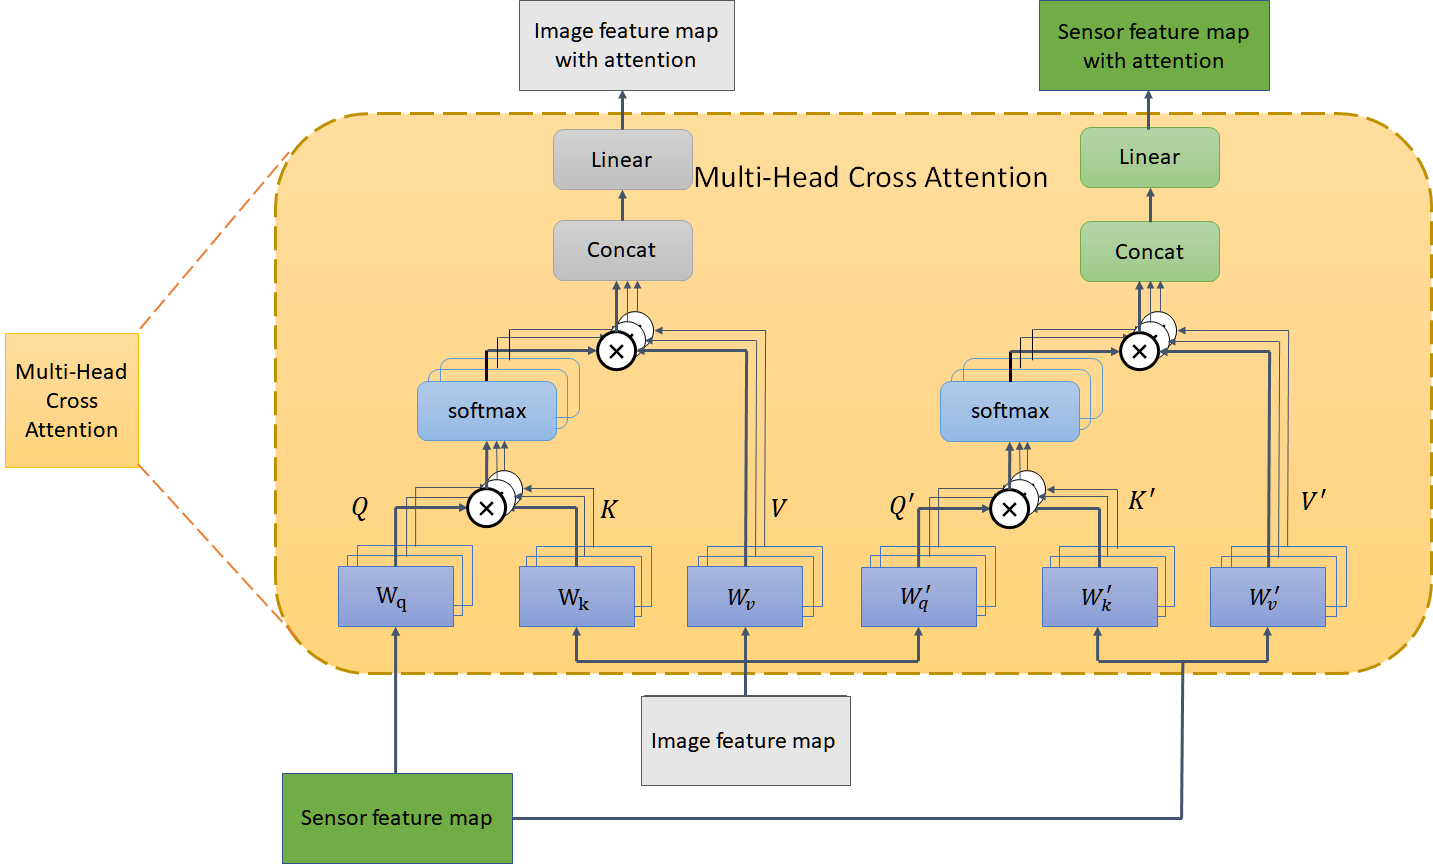
\includegraphics[width=\linewidth]{pic/cross_attention.png}
  \caption{Multi-Head Cross Attention Module structure.}
  \Description{Cross attention module in transformer.}
  \label{cross_attention}
\end{figure}
The Transformer Encoder for Fusion (TEF) module structure consists of multiple alternating layers of Multi-Head Cross Attention (MHCA, shown in Figure \ref{cross_attention}) and multiple MLP blocks. Layernorm (LN) is applied before every block in TEF. MLP module in TEF is referenced from ViT. The input of TEF is an Image Feature(IFM) for and Sensor Feature Map(SFM), and the output of TEF is a feature map of fusion. The calculation process is as follows.
\begin{equation}
  I_{attn},S_{attn}=MHCA\left(I_{in},S_{in}\right)
\end{equation}
\begin{equation}
  I_{out}=MLP\left(LN\left(I_{in}\cdot I_{attn}\right)\right)+I_{in}\cdot I_{attn}
\end{equation}
\begin{equation}
  S_{out}=MLP\left(LN\left(S_{in}\cdot S_{attn}\right)\right)+S_{in}\cdot S_{attn}
\end{equation}
where \begin{math}  I_{in}\end{math} is input of Feature map for image. \begin{math}
  I_{out}
\end{math} is the output of Feature Map. There are 12 layers of calculation for \begin{math}I_{out} \end{math}. The calculation method of \begin{math} S_{in}\end{math} and \begin{math}
  S_{out}
\end{math} is the same as \begin{math}
  I_{in}
\end{math} and \begin{math}
  I_{out}
\end{math}.\begin{math}
  I_{attn}
\end{math} is attention feature map of Image and \begin{math}
  S_{attn}
\end{math} is attention feature map of Sensor data.\begin{math}
  I_{out}
\end{math} and \begin{math}
  S_{out}
\end{math} are outputs of TEF. Finally, \begin{math}
  I_{out}
\end{math} , and \begin{math}
  S_{out}
\end{math} are spliced into the output of MM.

A key idea of this paper is to use MHCA to complete feature fusion. The Cross Attention mechanics is proposed to balance interactive effects between two features from image and sensor data.
Two part query the image and sensor feature maps for determining the parameters, respectively. The structure of MHCA is shown in Figure \ref{cross_attention}. One part takes the SFM as query(Q) and the IFM as the target of query to compute key(K) and value(V). The other part uses IFM as \begin{math}
  Q^\prime
\end{math}, the specific calculation formula is as follows.
\begin{equation}
  Q=SW_q,K=IW_k,V=IW_v
\end{equation}
\begin{equation}
  A=softmax\left(\frac{QK^T}{\sqrt{C/h}}\right)\ V
\end{equation}

\begin{equation}
  Q^\prime=I^\prime W_q^\prime,K^\prime=SW_k^\prime,V^\prime=SW_v^\prime
\end{equation}
\begin{equation}
  A^\prime=softmax\left(\frac{Q^\prime K^{\prime T}}{\sqrt{C/h}}\right)V^\prime
\end{equation}
where \begin{math}
  I
\end{math} is IFM and \begin{math}
  S
\end{math} is SFM. \begin{math}
  W_q,W_k,W_v\in R^{C\times\left(C/h\right)}
\end{math} are learnable parameters, \begin{math}
  C
\end{math} and \begin{math}
  h
\end{math} are the embedding dimension and number of heads.  Since a single modal feature map is used in the query, the computation and memory complexity of generating the attention map (\begin{math}
  A
\end{math} and \begin{math}
  A^\prime
\end{math}) in cross-attention are linear rather than quadratic as in all-attention. The entire process is more efficient. And it can reduce the risk of overfitting. In addition, multiple heads are used cross attention. Finally, features from multiple heads are spliced, and they are input for Linear to generate the output of MHCA.

\subsection{Loss function}
This paper adopted supervised learning, and actual LAI data manually collected from real farms oversee the learning. The loss function estimates the degree of inconsistency between the predicted value \begin{math}
  f(x)
\end{math} and the true value \begin{math}
  Y
\end{math} of the model. It is a non-negative real-valued function, usually expressed by \begin{math}
  L(Y, f(x))
\end{math}. The loss function is the core of the empirical risk function and an essential part of the structural risk function. 

In this paper, crop growth prediction is treated as a regression problem. The regression problem solves the prediction of specific values, such as house price prediction, sales prediction, etc. The neural network to solve the regression problem generally has only one output node, and the output value of this node is the predicted value. The loss function used under the regression problem is the mean square error loss function.
\begin{equation}
  MSE\left(y,y^\prime\right)=\frac{\sum_{i=1}^{n}\left(y_i-y_i^\prime\right)^2}{n}
\end{equation}
where \begin{math}
  n
\end{math} is the number of samples, \begin{math}
  y
\end{math} is the true value of the leaf area index, and \begin{math}
  y^\prime
\end{math} is the predicted value of the leaf area index. The mean square error was used to evaluate the accuracy of the model output and help the model update the parameters further.
\section{Experiments and Results}
In this part, we will introduce data collection, data collection equipment, and data format. Image and sensor data are preprocessed after data collection. The performance measures for evaluating the models and the experimental details are described.
\subsection{Study area and data}
Data include weather, soil, crop image, leaf area index, etc. The data were collected at Farm 290, Suibin County, Hegang City, Heilongjiang Province, China. The data acquisition location is shown in Figure \ref{farm_location}. The data were collected from three crops(rice, maize, and soybean). The data were collected from three sites for each crop. The data acquisition equipment is shown in Figure \ref{data_collection_equipment}. Cameras and sensors were placed in each area of the farm. LAI data were collected periodically using a hand-held device, taking multiple measurements each time to prevent accidental errors. The image and sensor data were collected in real-time and uploaded to the cloud server periodically for storage, which is convenient for remote viewing and data analysis.
\begin{figure}[htbp]
  \centering
  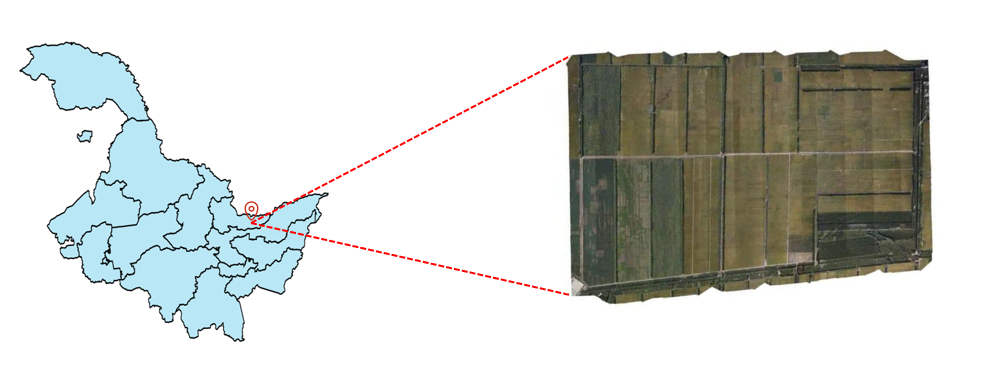
\includegraphics[width=\linewidth]{pic/farm_location.png}
  \caption{The location of the farm where data were collected.}
  \Description{Data collection farm location.}
  \label{farm_location}
\end{figure}

\begin{figure}[htbp]
  \centering
  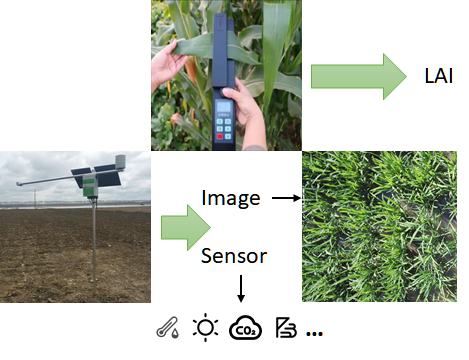
\includegraphics[width=0.5\linewidth]{pic/data_acquisition_equipment.png}
  \caption{Data acquisition equipment.}
  \Description{Data acquisition equipment.}
  \label{data_collection_equipment}
\end{figure}
\begin{figure}[htbp]
  \centering
  \subcaptionbox{Rice image data.}{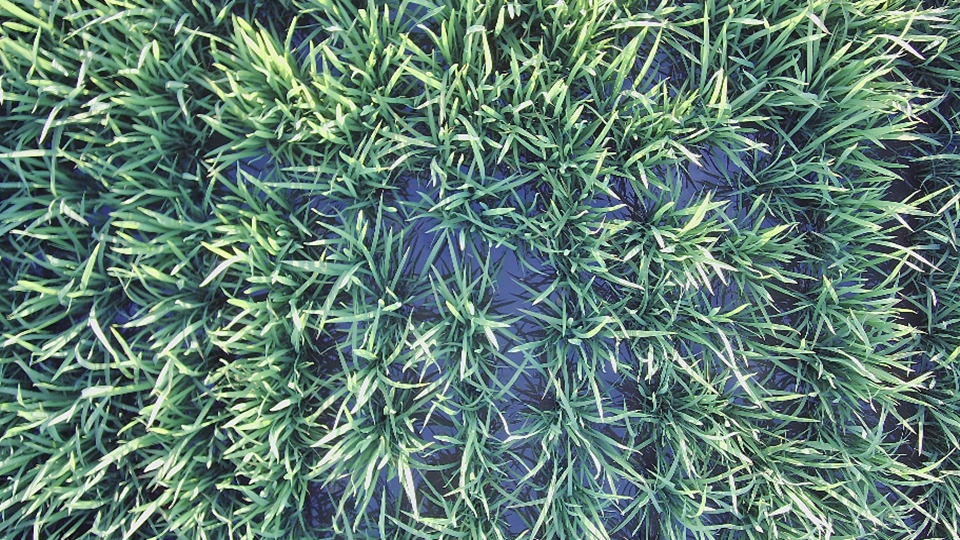
\includegraphics[width = 0.33\textwidth]{pic/rice.png}}
  \subcaptionbox{Soybean image data.}{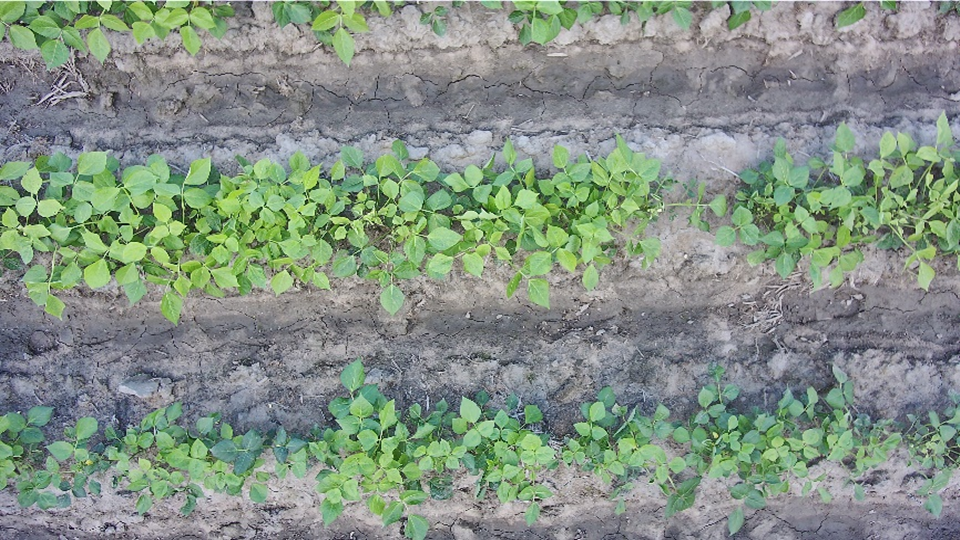
\includegraphics[width = 0.33\textwidth]{pic/soybean.png}}
  \subcaptionbox{Maize image data.}{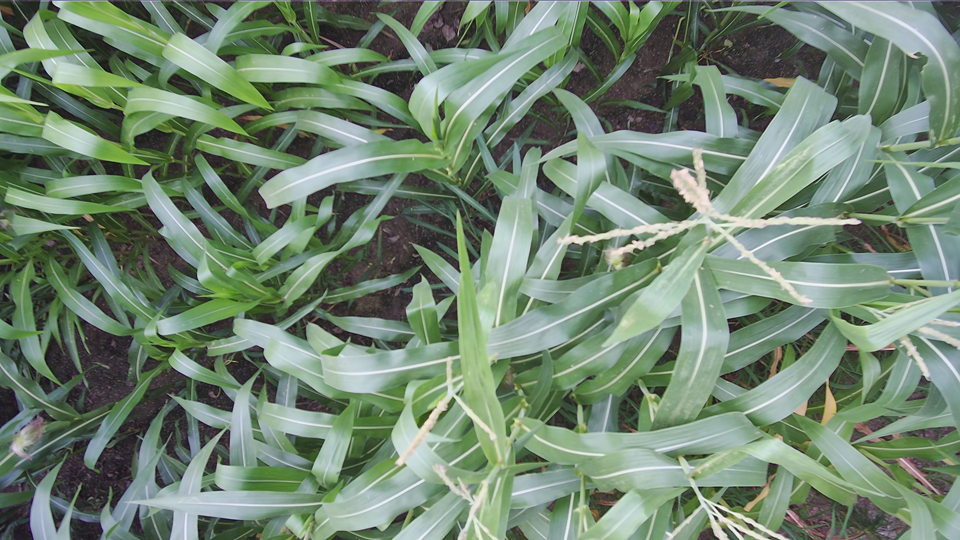
\includegraphics[width = 0.33\textwidth]{pic/corn.png}}\hfill
  % 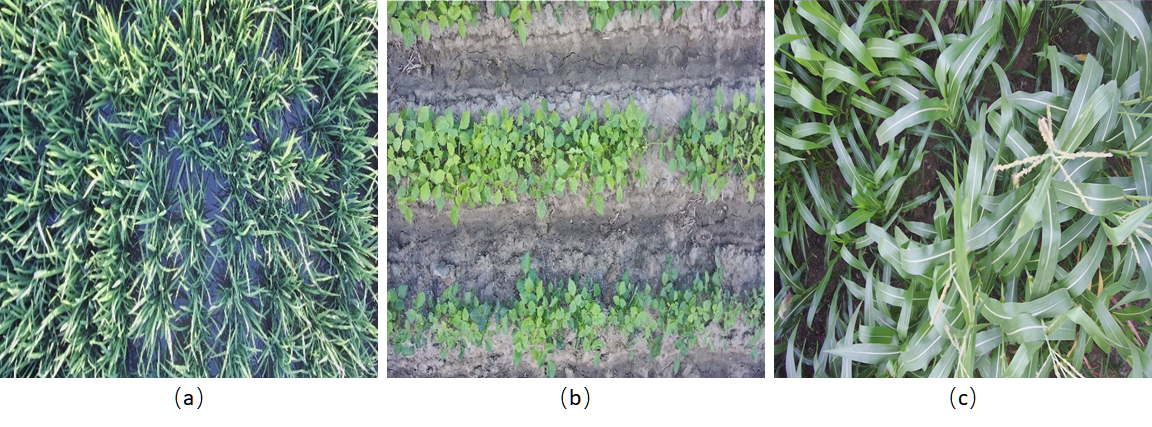
\includegraphics[width=\linewidth]{pic/crop.png}
  \caption{Crop image data.}
  \Description{Crop image data.}
  \label{crop} 
\end{figure}



Image acquisition takes the form of a fixed camera shot. The image format is RGB with a resolution of 3840\begin{math}
  \times
\end{math}2160. Three points are fixed for each crop, and the crops are photographed from a top view. The height is set at 3 meters. The time interval between each shot was two hours, and 12 RGB image data were taken by a single camera daily. The images of rice, soybeans, and maize captured by the camera on the farm are shown in Figure \ref{crop}(a)(b)(c), respectively.

The collected sensor data items are shown in Table \ref{tab:sensor_and_data_items}, which includes eleven sensor data types. The soil sensors were deployed in the ground at 10cm, 20cm, 30cm, 40cm, and 50cm depths, respectively. Sensors were deployed on the top of the IoT Device.


\begin{table*}
  \caption{Sensor data}
  \label{tab:sensor_and_data_items}
  \begin{tabular}{ll}
    \hline
    Data item & Unit \\
    \hline
    Carbon dioxide & PPM \\
    Soil temperature & Celsius \\
    Soil humidity & \% \\
    Air temperature & Celsius \\
    Air humidity & \% \\
    Light intensity & Klux \\
    Wind direction & degree \\
    Wind speed & Meters per second \\
    Air pressure & Hpa \\
    PM10  & PPM \\
    PM2.5 & PPM \\
    \hline
    \end{tabular}%
\end{table*}

\subsection{Data preprocessing}
\textbf{Preprocessing of sensor data:}The numerical differences of each dimension are relatively large for the sensor data. We used the following equation to perform normalization for each size to eliminate the influence of dimensions.

\begin{equation}
  y_{ij}=\frac{x_{ij}-min\left(x_j\right)}{max\left(x_j\right)-min\left(x_j\right)}\left(i=1,2,\ldots,n;j=1,2,\ldots,m\right)
\end{equation}
where \begin{math}
  min(x_j)
\end{math} is the minimum value of index \begin{math}
  x_j
\end{math}, and
\begin{math}
  max(x_j)
\end{math} is the maximum value of index \begin{math}
  x_j
\end{math}.

The maximum and minimum values for each metric were saved in a separate file for data preprocessing when they were used for processing actual data.The processed data are shown in Table \ref{tab:sensor_input_metrics_preprocessing}.


\begin{table*}
  \caption{Sensor input metrics preprocessing \label{tab:sensor_input_metrics_preprocessing}}

  \begin{tabular}{lll}
    \hline
    \multicolumn{1}{l}{Indicators} & \multicolumn{1}{l}{Minimum} & \multicolumn{1}{l}{Maximum} \\
    \hline
    Carbon dioxide & 364   & 636 \\
    Soil temperature for 10 centimeters depth & 18.1  & 25.1 \\
    Soil temperature for 20 centimeters depth & 18.3  & 23 \\
    Soil temperature for 30 centimeters depth & 18.3  & 22.1 \\
    Soil temperature for 40 centimeters depth & -30   & -30 \\
    Soil temperature for 50 centimeters depth & 17.1  & 21.2 \\
    Soil humidity for 10 centimeters depth & 46.8  & 80.6 \\
    Soil humidity for 20 centimeters depth & 53    & 75.6 \\
    Soil humidity for 30 centimeters depth & 55.2  & 79.5 \\
    Soil humidity for 40 centimeters depth & 0     & 80.6 \\
    Soil humidity for 50 centimeters depth & 67.3  & 81.5 \\
    Air humidity & 31    & 98.53 \\
    PM10  & 0     & 128 \\
    PM2.5 & 0     & 55 \\
    Air pressure & 981.1 & 1005.1 \\
    Light intensity & 0     & 200 \\
    Air temperature & 16.37 & 30.99 \\
    Wind direction & 0     & 359.8 \\
    Wind speed & 0     & 6.68 \\
    LAI   & 1.3075 & 1.91 \\
    \hline
    \end{tabular}%
\end{table*}
\textbf{Preprocessing of image data:}Image data were normalized to a specific range, ensuring better convergence in backpropagation. The Z-score method was used to normalize the data of each image.

\begin{equation}
  y=\frac{x-\mu}{\sigma}
\end{equation}
where \begin{math}
  \mu
\end{math} is the mean value, \begin{math}
  \sigma
\end{math} is the standard deviation, \begin{math}
  x
\end{math} is the input data, \begin{math}
  y
\end{math} is the output. The mean and standard deviation of the three channels of the image were recorded, respectively. The mean value of the normalized image on each channel was 0, and the variance was 1. This method did not apply to the case of a small sample size. Generally speaking, it can be used only when the sample size exceeds 30. The normalized results of image calculation for rice, soybean, and maize are shown in Table \ref{tab:image_standardized_data}.
\begin{table}[htbp]
  \caption{Image standardized data}
  \label{tab:image_standardized_data}
  \begin{tabular}{lllc}
    \toprule
    crop                                            & channel   & mean   & standard deviation \\
    \midrule
    \multicolumn{1}{c}{\multirow{3}[1]{*}{rice}}    & Channel 1 & 0.4452 & 0.1973             \\
                                                    & Channel 2 & 0.5014 & 0.2035             \\
                                                    & Channel 3 & 0.4292 & 0.183              \\
    \midrule
    \multicolumn{1}{c}{\multirow{3}[0]{*}{soybean}} & Channel 1 & 0.5    & 0.1517             \\
                                                    & Channel 2 & 0.5355 & 0.1641             \\
                                                    & Channel 3 & 0.487  & 0.1497             \\
    \midrule
    \multicolumn{1}{c}{\multirow{3}[1]{*}{corn}}    & Channel 1 & 0.4452 & 0.1973             \\
                                                    & Channel 2 & 0.5014 & 0.2035             \\
                                                    & Channel 3 & 0.4292 & 0.183              \\
    \bottomrule
  \end{tabular}
\end{table}


\textbf{Processing of LAI data:}Because the LAI data for each crop were collected manually, the time is not continuous, and the amount of data is relatively small. The piecewise cubic Hermite interpolation polynomial (PCHIP) method was used to obtain more LAI data.  The LAI data of rice, soybean, and maize were interpolated for each day, as shown in Figure \ref{lai}(a),(b),(c), respectively. In the figure, the left side is the original data, and the right is the interpolated data. From the curve, it can be seen that the interpolated image is smoother.

\begin{figure}[htbp]
  \centering
  \subcaptionbox{Before and after rice LAI interpolation \label{1}}{  \begin{minipage}{0.49\linewidth}
    \centering
    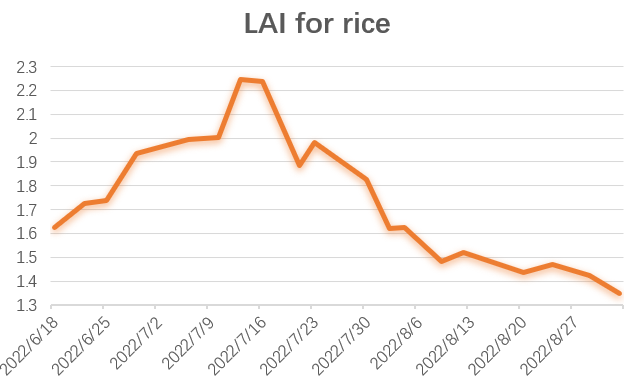
\includegraphics[width=\linewidth]{pic/rice_lai_before.png}
  \end{minipage}
  %\qquad
  \centering
  \begin{minipage}{0.49\linewidth}
    \centering
    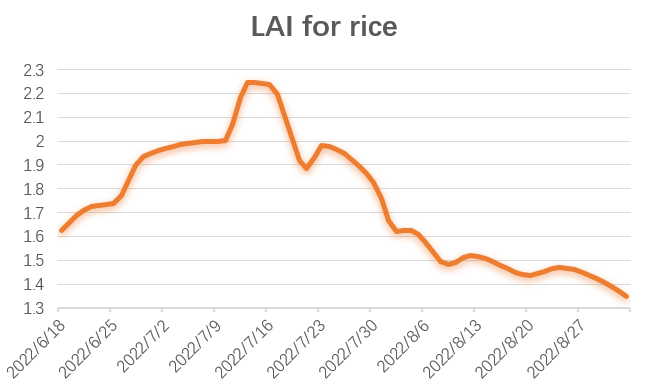
\includegraphics[width=\linewidth]{pic/rice_lai_after.png}
  \end{minipage}}\hfill

  \subcaptionbox{Before and after soybean LAI interpolation \label{2}}{  \begin{minipage}{0.49\linewidth}
    \centering
    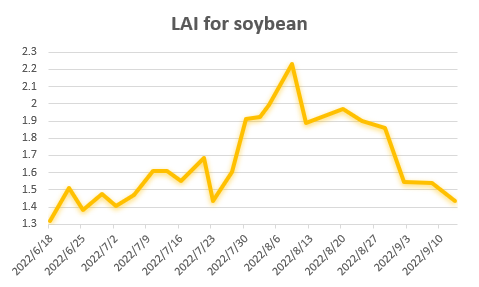
\includegraphics[width=\linewidth]{pic/soybean_lai_before.png}
  \end{minipage}
  %\qquad
  \centering
  \begin{minipage}{0.49\linewidth}
    \centering
    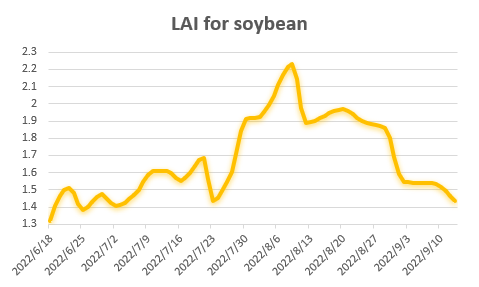
\includegraphics[width=\linewidth]{pic/soybean_lai_afterg.png}
  \end{minipage}}\hfill


  \subcaptionbox{Before and after maize LAI interpolation \label{3}}{  \begin{minipage}{0.49\linewidth}
    \centering
    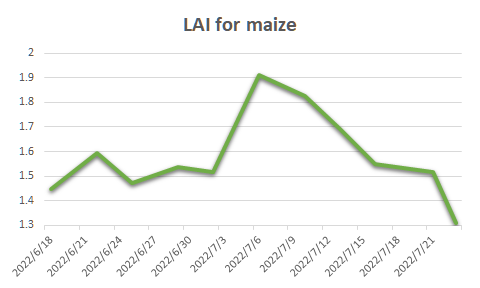
\includegraphics[width=\linewidth]{pic/corn_lai_before.png}
  \end{minipage}
  %\qquad
  \centering
  \begin{minipage}{0.49\linewidth}
    \centering
    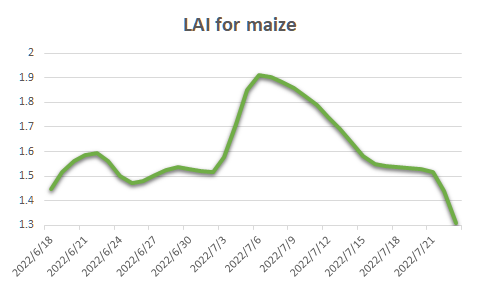
\includegraphics[width=\linewidth]{pic/corn_lai_after.png}
  \end{minipage}}\hfill
 \caption{LAI data preprocessing.}
 \Description{LAI data preprocessing.}
\label{lai}
\end{figure}

\textbf{Data alignment:} The leaf area index data were used as the label of each data to calculate the model error during training and validation. Image data and sensor data were aligned based on time, and all data simultaneously were merged into one training data. The time alignment was based on an hourly basis; there are 24 time points in a day, such as 1:00, 2:00,3:00, etc. There may be multiple training data at the same time point. Since the amount of image data was less than the sensor data, multiple training data records correspond to one image at a one-time point. For the leaf area index data, since it only had one data per day, the leaf area index was labeled with the training data in the unit of days when the data were aligned.


\textbf{Training and test sets:}To make the model evaluation more objective and reasonable, the data sets of rice, maize, and soybean were divided into a training set and test set, respectively. 80\% of the samples of each crop were used as the training set, 10\% samples were used as the validation set, and the remaining 10\% samples were used as the test set, which was invisible to the model. The only model inference was made during the test process, and model parameters were not updated according to the loss function.

\subsection{Comparison models}
We compared our model with existing DNNF1 and DNNF2, two multimodal models for soybean yield prediction [50]. The inputs to DNNF1 and DNNF2 were multimodal data such as crop canopy spectrum, multi-spectral thermal sensors, and crop surface texture features. For comparison, the inputs to DNNF1 and DNNF2 in our research were modified to make them the same as the input to our ViST model. Figure \ref{dnnf1_and_dnnf2_model} shows the inputs to the two existing models.

For the DNNF1 model, we used pre-fusion. The images were converted into feature vectors using the Linear Projection Flattened Patches module and flattened into one-dimensional vectors. The sensor data and the one-dimensional vector of the image were spliced and input into the DNNF1 multilayer perceptron. For the DNNF2 model, we used post-fusion. After processing, the data were trained by multilayer perceptron, and the outputs of the two-layer MLP were concatenated and then input into the three-layer MLP of DNNF2. The final output result of the model was an LAI value, which represented the growth of crops.



\begin{figure}[htbp]
  \centering
  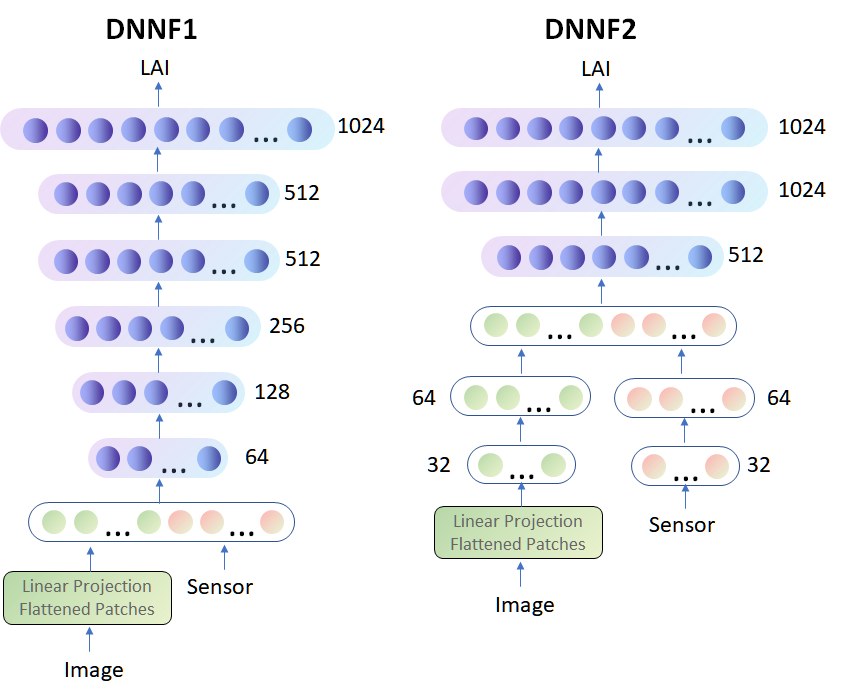
\includegraphics[width=0.8\linewidth]{pic/dnnf1_and_dnnf2_model.png}
  \caption{The structure of the models compared.}
  \Description{The structure of the models compared.}
  \label{dnnf1_and_dnnf2_model}
\end{figure}
\subsection{Evaluation Metrics}
Mean Absolute error (MAE) and mean square error (MSE) were used to evaluate the performance of various models where MSE is the same as the loss function. MAE is the sum of the absolute differences between the target and prediction values. It measures the average error size in a set of predicted values regardless of their direction and ranges from 0 to \begin{math}\infty\end{math}.
\begin{equation}
  MAE=\frac{\sum_{i}^{n}\left|y_i-y_i^p\right|}{n} \label{mae}
\end{equation}
where \begin{math}
  y_i^p
\end{math} is the predicted value of the model,\begin{math}
  y_i
\end{math} is the real value,
and \begin{math}
  n
\end{math} is the total number of samples.
One advantage of MAE over MSE is that it is less sensitive to outliers. Because MAE calculates the absolute value of the error,\begin{math}
  y-f\left(x\right)
\end{math}, the penalty is fixed for any different size.

The Mean Square Error (MSE) is the mean of the squared differences between the model's predicted value \begin{math}
  f(x)
\end{math}, and the actual sample value \begin{math}
  y
\end{math}. The formula is as follows:
\begin{equation}
  MSE=\frac{\sum_{i=1}^{n}\left(f_{x_i}-y_i\right)^2}{n}
  \label{mse}
\end{equation}
where \begin{math}
  y_i
\end{math} and \begin{math}
  f_{x_i},i
\end{math} are the true value and the corresponding predicted value for the first sample, and \begin{math}
  n
\end{math} is the number of samples

The leaf area index (LAI) was selected as an evaluation index of crop growth. The leaf area index (LAI) is a comprehensive index related to individual and group characteristics of crop growth \cite{__1999}. LAI cannot reflect all individual and group characteristics and must be supplemented by ground monitoring \cite{carlson_relation_1997}. Since images and sensors can provide adequate information on crop growth, images and sensors can be used as supplements to ground monitoring. After normalization, the leaf area index (LAI) ranges from [0,1].

\subsection{Experiments and results}
In this section, we describe extensive experiments conducted to show the effectiveness of our proposed ViST over existing methods. The experiments were introduced in two parts. First, we describe experimental results for a single crop. Second, we describe the experimental results for multiple crops. We performed ablation studies on ViST according to different input modes. The input modes were image-only data, sensor-only data, and multimodality data, respectively. The performance of each model was compared using MAE and MSE as given in Equations \ref{mae},\ref{mse}. 

The preprocessed data were used to train each model. The primary hyperparameters of ViST are given in Table \ref{tab:hyperparameters}. Adam optimizer was used, and the weight decay was set to 0.0001. All models were trained using a GeForce RTX 3090 GPU. The cosine annealing strategy was used to adjust the learning rate dynamically. The maximum number of iterations was adjusted according to the sample number and the epoch. Therefore, the learning rate was monotonically decreasing with increasing the number of epochs in the training process. The primary hyperparameters of the ViST model are shown in Table \ref{tab:hyperparameters}.  The parameters of each model were initialized using the random normal distribution. MM, SMI and SMS were used as the model's input for the ablation experiment. In all experiments, 80\%, 10\%, and 10\% of the dataset were used as the train, valid, and test data, respectively.


\begin{table}[htbp]
  \centering
  \caption{Main hyperparameters of the model}
  \begin{tabular}{ll}
    \toprule
    Parameter    & \multicolumn{1}{l}{Parameter size} \\
    \midrule
    hidden size  & 768                                \\
    head num     & 12                                 \\
    layer num    & 12                                 \\
    MLP ratio    & 4                                  \\
    drop rate    & 0.1                                \\
    sensor num   & 19                                 \\
    epoch        & 50                                 \\
    batch size   & 32                                 \\
    weight decay & 0.0001                             \\
    learning rate & 0.0001                             \\

    \bottomrule
  \end{tabular}%
  \label{tab:hyperparameters}%
\end{table}%

\subsubsection{Experiments and results for a single crop}

In this section, we tested our model for a single crop. We first compared the performance of the ViST model with single modality  data and multimodality data(see Section A). Then we compared the performance of the ViST model with other models(see Section B).

\textbf{A.}	Performance Comparison  of ViST model with single modality data and multimodality data

The ViST model was trained for a single crop with three different data input modes:  the first was trained using the image-only data; the second was trained using the sensor data only; the third was training using both of image and sensor data. Thus, three trained models were obtained for each crop.

Figure \ref{Rice_ViST_results} shows the validation information of the model trained using three different modes for rice. From Figure \ref{Rice_ViST_results}, we can find that the values of MAE and MSE decreased with the increase in the training rounds. When the input mode for the ViST model was multimodality, the lowest values of MSE and MAE were obtained when the model converged. The minimum MSE of the model with multimodality input mode reached 0.001044, which reduced the error by 52.35\%, and 84.62\% compared to image-only and sensor-only modes. The minimum MAE value of the model with multimodality input mode  reached 0.01999. The MAE of the Model with multimodality input mode was also significantly improved. The error of the MAE was reduced by 64.09\% and 39.24\% compared to sensor-only and image-only modes, respectively. It can be concluded that multimodal fusion helped performance improvement for crop growth prediction. Figure \ref{Soybean_ViST_results} and Figure \ref{maize_vist_results} show the training information of the model trained using three different modes for Soybean and Maize, respectively. We obtained similar results, which show that training results with multimodality input mode had the lowest MAE and MSE values when the network converged. In addition, the training with multimodality input mode had the fastest convergence speed.

   \begin{figure}[htbp]
    \centering
    \begin{minipage}{0.49\linewidth}
      \centering
      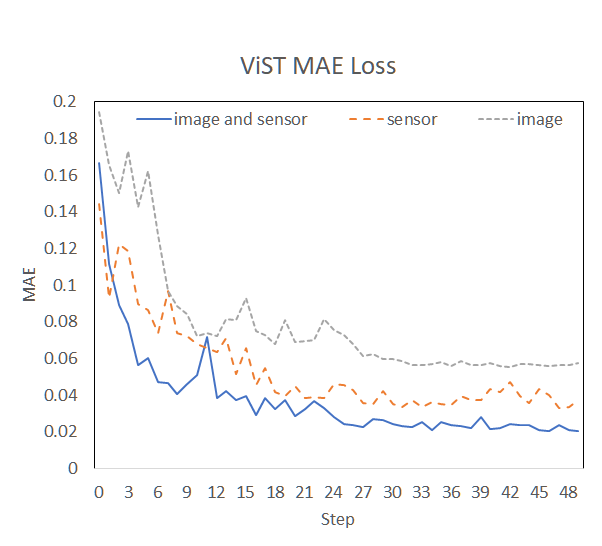
\includegraphics[width=\linewidth]{pic/res_rice_vist_mae.png}
    \end{minipage}
    %\qquad
    \centering
    \begin{minipage}{0.49\linewidth}
      \centering
      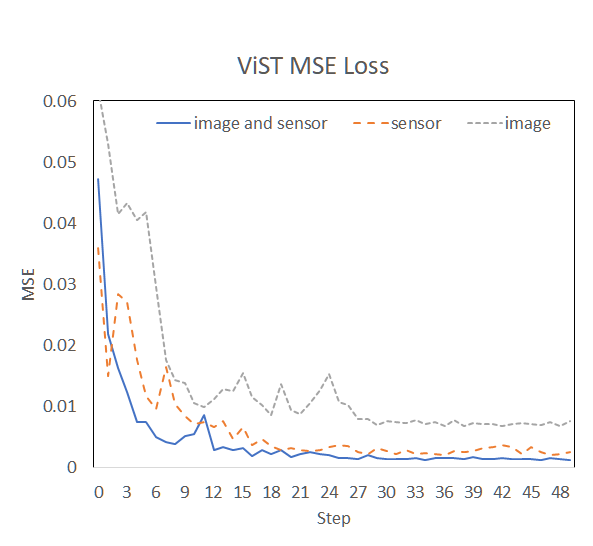
\includegraphics[width=\linewidth]{pic/res_rice_vist_mse.png}
    \end{minipage}
    \caption{ViST model for rice training results for different input modes. \label{Rice_ViST_results}}
    \Description{ViST model for rice training results for different input modes.}
  \end{figure}


  \begin{figure}[htbp]
    \centering
    \begin{minipage}{0.49\linewidth}
      \centering
      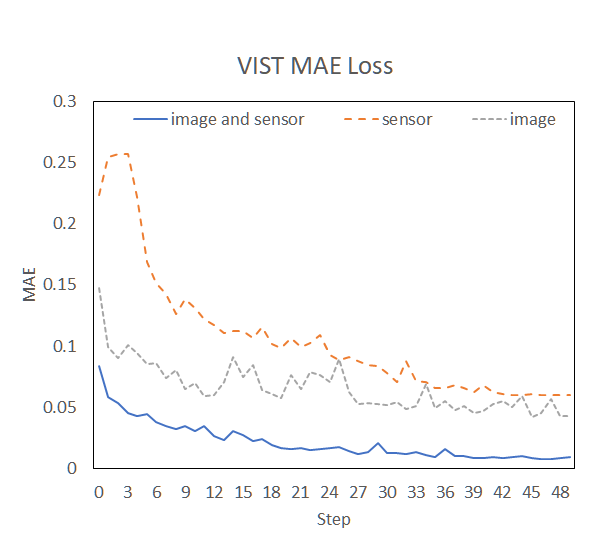
\includegraphics[width=\linewidth]{pic/res_soybean_vist_mae.png}
    \end{minipage}
    %\qquad
    \centering
    \begin{minipage}{0.49\linewidth}
      \centering
      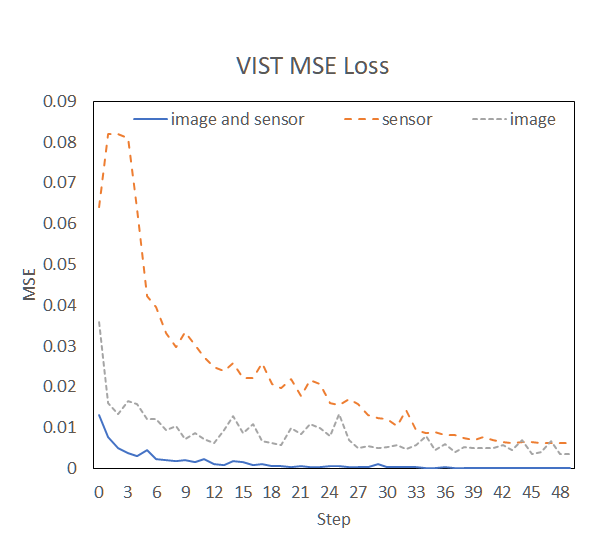
\includegraphics[width=\linewidth]{pic/res_soybean_vist_mse.png}
    \end{minipage}
  
    \caption{Soybean ViST model training results for different modes. \label{Soybean_ViST_results}}
    \Description{Soybean ViST model training results for different modes.}
  \end{figure}

  \begin{figure}[htbp]
    \centering
    \begin{minipage}{0.49\linewidth}
      \centering
      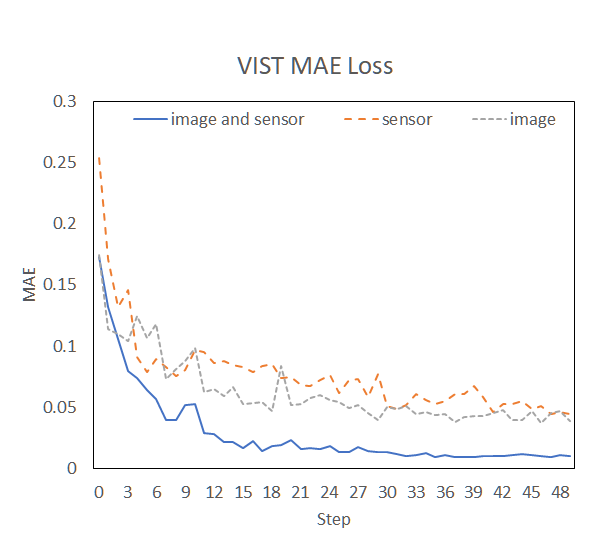
\includegraphics[width=\linewidth]{pic/res_corn_vist_mae.png}
    \end{minipage}
    %\qquad
    \centering
    \begin{minipage}{0.49\linewidth}
      \centering
      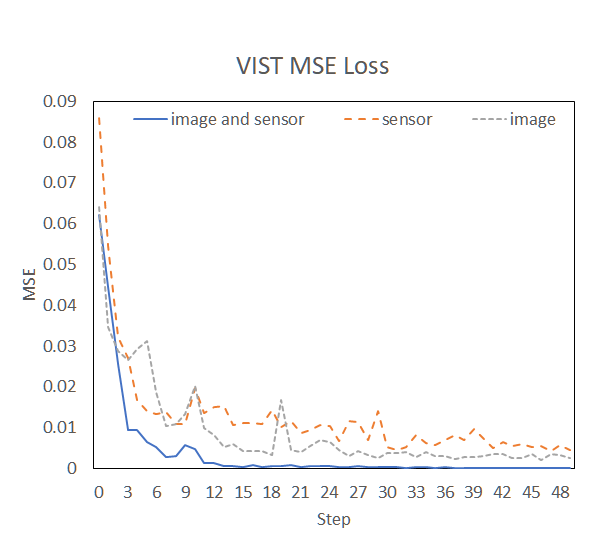
\includegraphics[width=\linewidth]{pic/res_corn_vist_mse.png}
    \end{minipage}
  
    \caption{Maize ViST model training results for different input modes. \label{maize_vist_results}}
    \Description{Maize ViST model training results for different input modes.}
  \end{figure}

  % Table generated by Excel2LaTeX from sheet 'Sheet1'
\begin{table}[htbp]
  \centering
  \caption{ViST model test results for different input modes.}
    \begin{tabular}{llllll}
    \hline
    \multicolumn{1}{l}{\multirow{2}[4]{*}{Crop}} & \multicolumn{1}{l|}{\multirow{2}[4]{*}{Input mode}} & \multicolumn{2}{p{8.38em}|}{{Validation}} & \multicolumn{2}{p{8.38em}}{{Test}} \\
\cline{3-6}          & \multicolumn{1}{l|}{} & \multicolumn{1}{p{4.19em}}{{MAE}} & \multicolumn{1}{p{4.19em}|}{{MSE}} & \multicolumn{1}{p{4.19em}}{{MAE}} & \multicolumn{1}{p{4.19em}}{{MSE}} \\
    \hline
    \multicolumn{1}{l}{\multirow{3}[1]{*}{rice}} & Image & 0.05566 & 0.00679 & 0.05764 & 0.007581 \\
          & Sensor & 0.0329 & 0.002191 & 0.03707 & 0.002595 \\
          & Multimodality & 0.01999 & 0.001044 & 0.02012 & 0.00123 \\
    \multicolumn{1}{l}{\multirow{3}[0]{*}{soybean}} & Image & 0.04185 & 0.003567 & 0.04254 & 0.003638 \\
          & Sensor & 0.05961 & 0.006247 & 0.05974 & 0.006251 \\
          & Multimodality & 0.007779 & 0.000117 & 0.009076 & 0.000158 \\
    \multicolumn{1}{l}{\multirow{3}[1]{*}{maize}} & Image & 0.03698 & 0.002112 & 0.03844 & 0.002527 \\
          & Sensor & 0.04475 & 0.004377 & 0.04455 & 0.004638 \\
          & Multimodality & 0.009159 & 0.000223 & 0.01053 & 0.000201 \\
    \hline
    \end{tabular}%
  \label{tab:vist_model_test_results}%
\end{table}%

  After the trained models were obtained, we used the data from the test dataset to test the models.
  The performance of the ViST model with single modality data and multimodality data for validation dataset and test dataset is shown in table \ref{tab:vist_model_test_results}. The model obtained using Multimodality data achieved the best performance in three input modes for each crop. Soybean had the best performance. The MSE of soybean for the test dataset reached 0.000158, which reduced the error by 97.47\%, and 95.66\% in comparison with image data only and sensor data only mode. The error of the MAE was reduced by 84.81\% and 78.66\% compared with sensor-only data and image-only data, respectively. Obviously, multimodality can bring higher accuracy to the model. The performance of rice was the worst among the three crops. But the performance obtained by multimodality data mode also had a good performance. The MSE value of the model with multimodality data mode for rice obtained by the test dataset reached 0.00123, which reduced the error by 52.60\%, and 46.30\% in comparison with sensor-only data and image-only data. The error of the MAE was reduced by 45.72\% and 65.09\% in comparison with sensor-only data and image-only data. Therefore, the performance with multimodality data mode is better than that of single mode for the same crop.


\textbf{B.Comparison with DNNF1 and DNNF2:}
In this Section, we compared the proposed ViST model with two other popular models: DNNF1, and DNNF2. All three models were trained on rice, soybean, and maize data, respectively. Experimental results show that the Loss of the ViST with multimodal input had the lowest value compared with that of DNNF1 and DNNF2 in almost all of the cases. Therefore, the Transformer-based ViST has apparent advantages over DNNF1 and DNNF2.
\begin{figure}[htbp]
  \centering
  \begin{minipage}{0.49\linewidth}
    \centering
    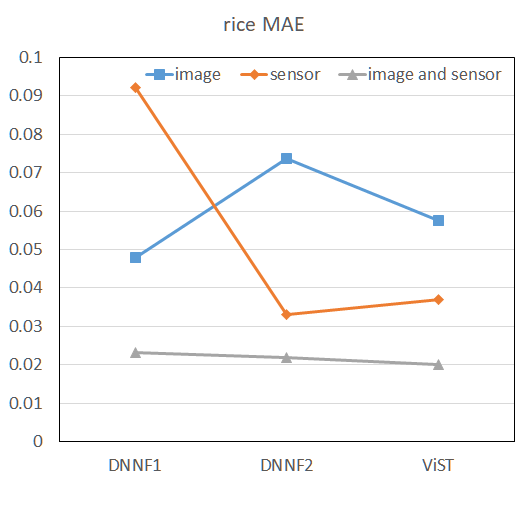
\includegraphics[width=\linewidth]{pic/comprehensive_rice_mae.png}
  \end{minipage}
  %\qquad
  \centering
  \begin{minipage}{0.49\linewidth}
    \centering
    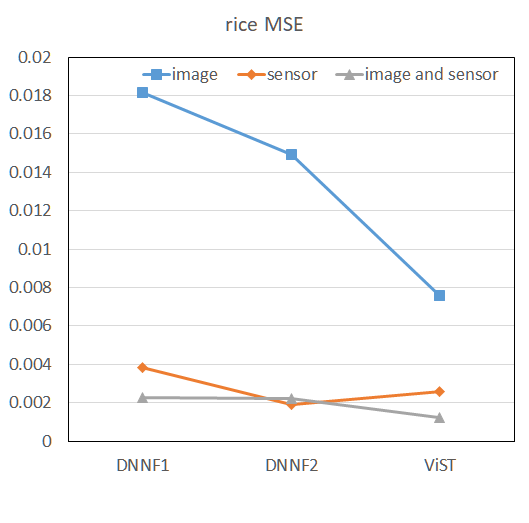
\includegraphics[width=\linewidth]{pic/comprehensive_rice_mse.png}
  \end{minipage}

  \caption{Comprehensive comparison of three models for rice. \label{comprehensive_rice}}
  \Description{Comprehensive comparison of models for rice .}
\end{figure}

Figure \ref{comprehensive_rice} shows the experimental results for rice.  Although the performance of the proposed ViST model didn't have the best performance for single input modes, the proposed ViST model had the lowest MAE and MSE values for multiple models mode. From the perspective of MAE, the loss of ViST with multimodal input reaches 0.02012, which reduced the error by 13.39\%, and 8.30\% compared with DNNF1 and DNNF2, respectively. From the perspective of MSE, the loss of ViST with multimodal input reached 0.00123, which reduces the error by 46.41\% and 44.94\% compared with DNNF1 and DNNF2, respectively. 

\begin{figure}[htbp]
  \centering
  \begin{minipage}{0.49\linewidth}
    \centering
    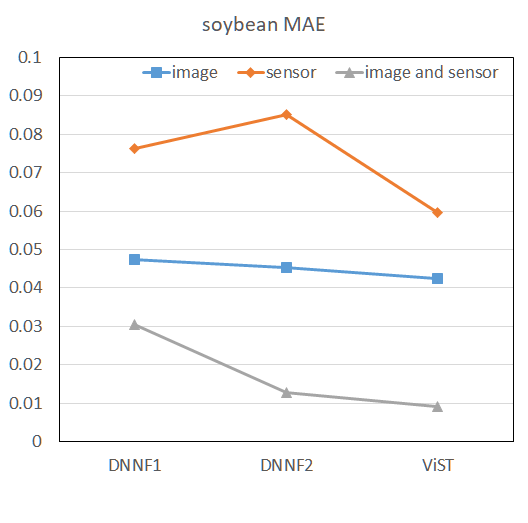
\includegraphics[width=\linewidth]{pic/comprehensive_soybean_mae.png}
  \end{minipage}
  %\qquad
  \centering
  \begin{minipage}{0.49\linewidth}
    \centering
    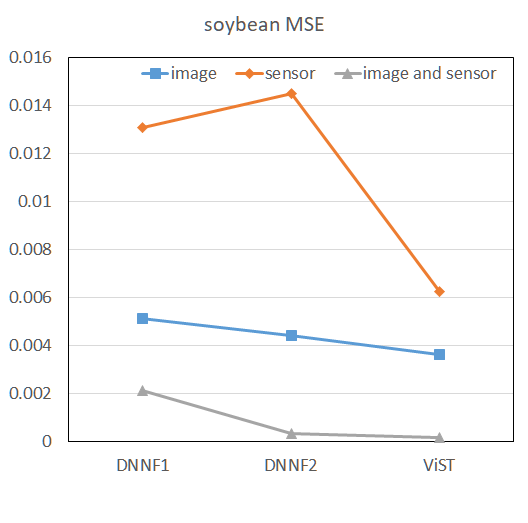
\includegraphics[width=\linewidth]{pic/comprehensive_soybean_mse.png}
  \end{minipage}

  \caption{Comprehensive comparison of three models for soybean. \label{comprehensive_soybean}}
  \Description{Comprehensive comparison of models for soybean .}
\end{figure}

Figure \ref{comprehensive_soybean} shows the comprehensive comparison of three models for soybean. ViST performed best under all three input modes. The DNNF2 model outperformed DNNF1 with image-only and multimodal input modes. DNNF1 performed better than DNNF2 with sensor-only mode. For MAE, the error of the ViST reached 0.009076, which reduced the error by 70.20\% a   29.26\% compared with DNNF1 and DNNF2, respectively. From the perspective of MSE, the error of ViST reached 0.000158, which reduced the error by 92.60\%, and 51.29\% compared with DNNF1 and DNNF2, respectively. The ViST had a greater improvement in performance than DNNF1 and DNNF2, and DNNF2 was better than DNNF1. The accuracy improvement of the ViST model is relatively significant, and the robustness is better under the condition of multimodal input mode.


\begin{figure}[htbp]
  \centering
  \begin{minipage}{0.49\linewidth}
    \centering
    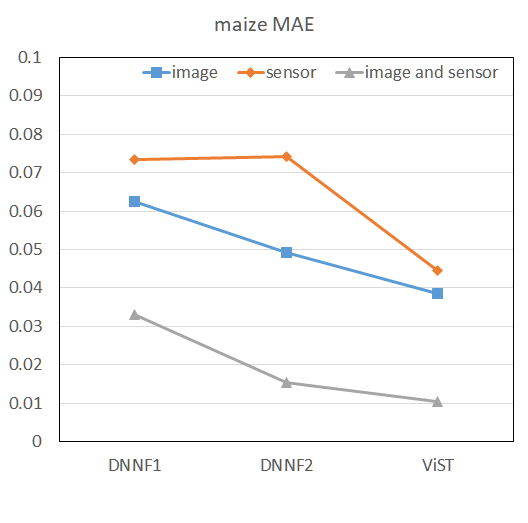
\includegraphics[width=\linewidth]{pic/comprehensive_corn_mae.png}
  \end{minipage}
  %\qquad
  \centering
  \begin{minipage}{0.49\linewidth}
    \centering
    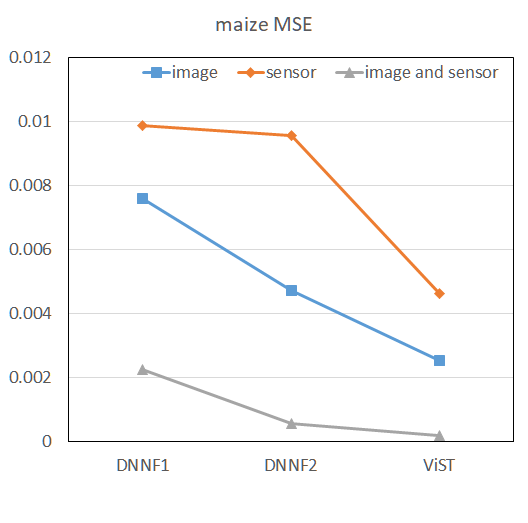
\includegraphics[width=\linewidth]{pic/comprehensive_corn_mse.png}
  \end{minipage}

  \caption{Comprehensive comparison of three models for maize. \label{comprehensive_maize}}
  \Description{Comprehensive comparison of  models for corn.}
\end{figure}

The comprehensive comparison of their models for Maize is shown in Figure \ref{comprehensive_maize}, and the ViST model performed best in all of the three input modes. The accuracy and stability of the DNNF2 model were higher than those of DNNF1. From  MAE, the error of ViST reached 0.01053, which reduced the error by 68.04\% and 31.98\% compared with DNNF1 and DNNF2, respectively. From MSE, the error of ViST reached 0.0002008, which reduced the error by 91.03\% and 63.54\% compared with DNNF1 and DNNF2, respectively. Therefore, ViST has good precision and stability on Maize data.

\subsubsection{Experiments and results for hybrid network training}

The data from three crops were mixed and used to train the model to test the model's generalization ability for the growth prediction of multiple crops. The results of ViST, DNNF1, and DNNF2 models with the hybrid data set as input are shown in Figure \ref{hybrid_result}. It can be seen that the ViST models still had high accuracy compared with the other two models when multiple crops were mixed as the input to train the model. The convergence speed of MAE and MSE loss for the ViST model was significantly faster than that of DNNF1 and DNNF2.  Under 50 training iterations, the MSE loss of ViST reached 0.0005848 when the model converged, which reduced the error by about half compared with DNNF1 and DNNF2. For MAE, the ViST model had the least value compared with DNNF1 and DNNF2 when the model converged.
\begin{figure}[htbp]
  \centering
  \begin{minipage}{0.49\linewidth}
    \centering
    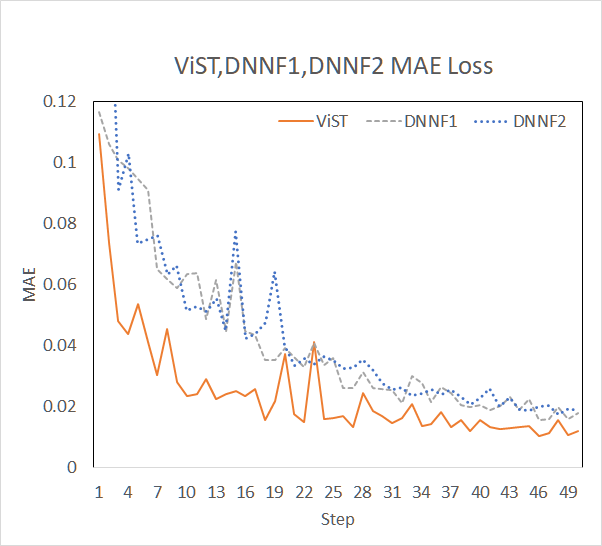
\includegraphics[width=\linewidth]{pic/generalization_vist_dnnf1_dnnf2_mae.png}
  \end{minipage}
  %\qquad
  \centering
  \begin{minipage}{0.49\linewidth}
    \centering
    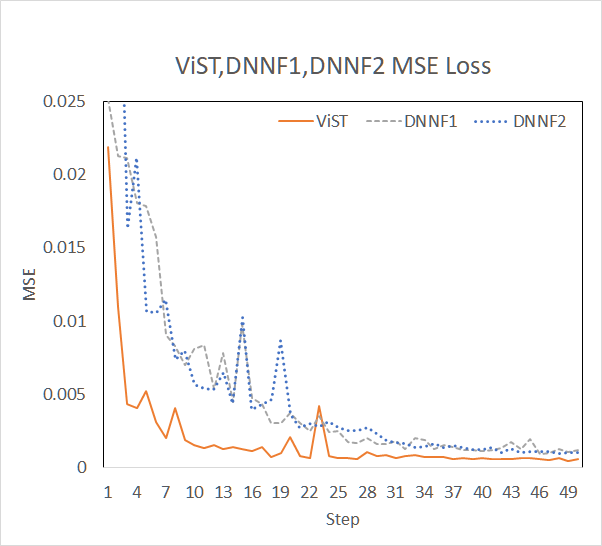
\includegraphics[width=\linewidth]{pic/generalization_vist_dnnf1_dnnf2_mse.png}
  \end{minipage}

  \caption{Comparison of ViST, DNNF1, DNNF2 models for three crops. \label{hybrid_result}}
  \Description{Comparison of ViST, DNNF1, DNNF2 models for three crops.}
\end{figure}

The results on the ubiquitous ability of ViST are shown in Table \ref{tab:ubiquitous}. When training and testing were from the same crop, the mean values of MAE were 0.02012, 0.009076, and 0.01053 for rice, maize and soybean, respectively. The MAE value obtained by hybrid training was 0.01198. When training and testing were from the same crop, the mean values of MSE were 0.00123, 0.000158, and 0.000201 for rice, Maize, soybean respectively. The MAE value obtained by hybrid training was 0.000585. From these numbers, we find that the errors obtained by training a hybrid network for multiple crops were similar to  the errors obtained by training a single network for a single crop. 


% Table generated by Excel2LaTeX from sheet 'Sheet1'
\begin{table}[htbp]
  \centering
  \caption{Comparison Results of ViST model with different crops as input.}
    \begin{tabular}{llll}
    \hline
    Train data & Test data & \multicolumn{1}{p{4.19em}}{MAE} & \multicolumn{1}{p{4.19em}}{MSE} \\
    \hline
    Rice  & Rice  & 0.02012 & 0.00123 \\
    Maize & Maize & 0.009076 & 0.000158 \\
    Soybean & Soybean & 0.01053 & 0.000201 \\
    Three crops & Three crops & 0.01198 & 0.000585 \\
    
    \hline
    \end{tabular}%
  \label{tab:ubiquitous}%
\end{table}%

\section{Conclusion and future work}
This paper proposed ViST, a Transformer-based model for crop growth prediction on a farm. The attention mechanism in the model was used to improve the effect of model fusion. The data of the three crops were trained together as input to the model. The model has high accuracy and good generalization ability. Experiment results show that the model with multimodality data can improve crop growth prediction. The data sets of various crops will be enriched to improve the model's prediction accuracy from the perspective of improving data quality.

We also show that it is possible to train a hybrid network for multiple crops. We will further investigate this issue in the future.
%%
%% The acknowledgments section is defined using the "acks" environment
%% (and NOT an unnumbered section). This ensures the proper
%% identification of the section in the article metadata, and the
%% consistent spelling of the heading.
\begin{acks}
  This research is supported by Heilongjiang NSF funding, No. LH202F022, Heilongjiang research and application of key technologies, No. 2021ZXJ05A03, and New generation artificial intelligent program, No.21ZD0110900 in CHINA.
\end{acks}

%%
%% The next two lines define the bibliography style to be used, and
%% the bibliography file.
\bibliographystyle{ACM-Reference-Format}
\bibliography{sample-base}


%%
%% If your work has an appendix, this is the place to put it.
\appendix



\end{document}
\endinput
%%
%% End of file `sample-acmsmall.tex'.
